\documentclass[12pt]{scrartcl}
\usepackage{amsmath,amssymb,amsthm}
\usepackage{ textcomp }
\usepackage{graphicx}
\usepackage[utf8]{inputenc}
\graphicspath{ {/TexmakerMacosxLion/} }
\usepackage{geometry}
\usepackage{pageslts}
\newenvironment{definition}[1][Definition]{\begin{trivlist}
\item[\hskip \labelsep {\bfseries #1}]}{\end{trivlist}}
\newenvironment{example}[1][Example]{\begin{trivlist}
\item[\hskip \labelsep {\bfseries #1}]}{\end{trivlist}}
\newenvironment{remark}[1][Remark]{\begin{trivlist}
\item[\hskip \labelsep {\bfseries #1}]}{\end{trivlist}}
\usepackage{graphicx}
\usepackage{fancyhdr}
\pagestyle{fancy}
\pagenumbering{arabic}
\rhead{Page {\thepage} of \lastpageref{LastPages}}
\lhead{Team \# 54642}

%\renewcommand{\headrulewidth}{0pt}

\usepackage[rightcaption]{sidecap}
 
\usepackage{graphicx} %package to manage images
 
 
 \title{Relieving the Space Jam}
 \subtitle{Assessment of a Quick-Response Satellite Mission to Neutralize Debris from Orbital Fragmentation Events}
 \author{Team \# 54642}
 \date{February 1, 2016}

\begin{document}


\maketitle

\newpage

%\begin{center}
%\includegraphics{.jpg}\\
%\textbf{Figure 1. }Figure caption text
%\end{center}

% TABLE IS HERE
\tableofcontents
\newpage

%\begin{center}
%\includegraphics[scale=0.4]{}\\
%\textbf{Figure #.} Put figure caption here.
%\end{center}

\section{Summary}

Over the course of the Space Age, human activity has left a large amount of debris in orbit around the Earth. Although some of this debris is decommissioned satellites and left-behind rocket parts, the vast majority of debris in orbit is due to satellite explosion and collision events \cite{ODPO}. These events generate large clouds of debris fragments, which although individually minuscule in size, threaten other spacecraft due to their kinetic energy. (A 1 kg object moving at normal low earth orbit speeds, packs the punch of a 35,000 kg truck moving at 190 km/h \cite{punch}!) \par
We set out to assess the feasibility of deploying a rapid-response satellite mission, SORES, to clean up the debris cloud from a fragmentation event before it can disperse. Through our models of satellite fragmentation and the orbital mechanics of debris dispersion, we assess the potential of such a mission to de-orbit debris. Our primary experimental variables are the fragmentation event-to-launch delay and effective radius of SORES (the range at which SORES de-orbits debris). We then consider the risks and economic viability of such a mission. The structure of our paper is as follows.

\begin{itemize}
    \item Our executive summary, Section \ref{sec:executive_summary}, provides a more detailed overview of our model, our results, and our recommendations. This section is targeted to a policy-making, administrative audience.
    \item Section \ref{sec:introduction} provides a detailed background to the history and science of space debris and motivates our paper.
    \item Sections \ref{sec:assumptions} and \ref{sec:vars_defns} describe the assumptions and variables behind our model and defines the standard simulation conditions that we adopted.
    \item We present our models for orbital mechanics and satellite fragmentation in Section \ref{sec:the_model}. We perform sensitivity analysis of our model in Section \ref{sec:sensitivity_analysis}. Later, in Section \ref{sec:model_assessment}, we assess the strengths and weaknesses of our model and identify potential improvements to it.
    \item We share the results of experiments performed with our models in Section \ref{sec:results}. 
    \item Section \ref{sec:discussion} provides risk and cost assessments of a SORES mission and discusses potential mechanisms by which SORES might de-orbit debris in light of our findings.
    \item Finally, Section \ref{sec:recommendations} ties together our findings into actionable recommendations to policymakers. 
\end{itemize}

\section{Executive Summary} \label{sec:executive_summary}
The \textbf{proliferation of space debris} poses a fundamental threat to global telecommunication, earth-monitoring research, and--most distressingly--human spaceflight activities. At current debris levels, collisions are rare and, to a large extent, can be avoided through vigilant monitoring and occasional orbital adjustments. However, once the density of space debris surpasses a threshold concentration, space debris have the \textbf{potential for explosive, exponential growth} through a chain reaction of collision events \cite{1995 IA}. NASA and the ESA estimate that it will be necessary to de-orbit ten ``high value'' pieces of space junk every year in order to prevent such a scenario from unfolding \cite{ESA}. We propose the implementation of a \textbf{fast-response countermeasure to orbital fragmentation events}: Space Orbit REmoval Satellite, which we affectionately call SORES. We do not propose a specific mechanism by which a SORES satellite might de-orbit space debris (although we do consider several mechanisms proposed by other groups in light of our findings).

In this paper, we assess the \textbf{potential effectiveness}, as well as the \textbf{potential cost and risk}, of a SORES intervention. Our team has created a mathematical model to \textbf{simulate debris fragmentation and the interaction of SORES} with those debris in orbit. Our model suggests that only a short delay between the fragmentation event and SORES launch is key to a successful cleanup mission. Our models suggest that a SORES mission launched just one day after a fragmentation event might be able to neutralize as much as 95 \% of the material generated by that event. With a one week fragmentation-to-launch time-frame, the amount of material neutralized by a SORES mission drops to slightly over 20 \%. We also find that a SORES satellite should have a radius of effect of at least around 1 km for the cleanup mission to be effective. Such an effective radius could potentially be implemented through a solar sail-type device or a deploy-able debris net coupled with an active guidance system or by a ranged mechanisms such as gas puffs or lasers \cite{tether} \cite{sail} \cite{net}. 

The results of our cost and risk assessment, however, are less promising. The largest risk of the project, in our estimation, is damage to SORES caused by the space debris that it is attempting to neutralize. To maximize the interaction of SORES with debris (hopefully leading to more debris being de-orbited), we propose that SORES be placed in the same orbit as the debris but travel in the opposite direction as the debris. Although, our simulations found that close passes to SORES (\(<\)10 m) by debris are unlikely, the potential for such an event does exist and this risk needs to be assessed further. The outcome of such a collision, of course, depends on the construction of SORES itself. \textbf{A robust, maneuverable satellite will be necessary for a SORES-type mission.} We find that a SORES mission has high costs, as well as high risks. We estimate that insurance companies pay out at most \$774 million annually to cover damage caused to satellites by debris. We used this number to estimate an upper bound on the unit value of de-orbiting debris: \$2,050 per debris neutralized. On average, a fragmentation event releases only 114 pieces of debris \cite{excel}. With total costs for a SORES mission at approximately \$200 million, a SORES approach to space junk removal simply does not pen out as a profitable endeavor at this time.

To summarize, we have found that, with an \textbf{optimistic launch schedule and a large radius} of debris de-orbit effectiveness, a SORES cleanup mission might be technically feasible. However, we find that under current conditions, such an intervention is not economically viable. The potential for exponential growth of debris through chain-collision events and decreased mission costs due to space-privatization revolution might tip the scales towards viability of SORES in the future.

\section{Introduction} \label{sec:introduction}
\subsection{Motivation}
Since the first man-made object reached space in the mid 1900's, countries all around the world have launched thousands of spacecraft including satellites, shuttles and probes \cite{ODPO}. When the functional lifespan of these objects is over or they become unresponsive for some reason, they are reduced to uncontrolled debris. Unlike a passing high-velocity meteoroid, the debris remains in orbit around the Earth until gravity pulls it close enough to the earth for it encounter particles of the atmosphere, resulting in drag. Compared to the high velocity orbit, drag causes a rapid deceleration leading to the eventual de-orbit of the object. The debris burns and is usually destroyed when it hits the atmosphere, but occasionally will reach the surface of the earth.

Such a de-orbiting process takes a number of years to occur naturally, depending on the original altitude. Due to the slow orbital decay of debris, there are a rapidly growing number of uncontrolled objects in orbit around the Earth. This has lead to many explosions and collisions, each one creating dust clouds with many smaller fragments traveling at very high velocities \cite{UN}. To illustrate, 1 kg object moving at normal low earth orbit speeds packs the punch of a 35,000 kg truck moving at 190 km/h \cite{punch}! Each piece of debris not only poses the risk of damage to passing spacecraft but has the potential to collide with other debris, thus creating a cascading effect. At the end of the 20th century, over 35 million pieces of debris were present in Earth Orbit \cite{1995 IA}. This number is growing exponentially, and with it grows the probability of damage to functional spacecraft \cite{UN}.

Of the total amount of cataloged debris in orbit around the Earth, approximately \(72\)\footnote{This total takes into account the debris smaller than 10 cm that is statistically estimated by damage to spacecraft because it is too small to be seen by radar.} \(\% \) is in the Lower Earth Orbit (LEO), which is defined as altitudes less than 2000 km \cite{1995 IA}. While the distribution of debris is very far from uniform, LEO contains the highest concentrations of debris at a density of \(4.55 \times 10^{-8}\) debris fragments per cubic kilometer. In particular, debris is most concentrated around 900 km altitude \cite{fragments}. 

\subsection{Debris Removal Strategies}
NASA and the European Space Agency state that an active debris removal strategy is most efficient if it is assessed in terms of the collisions prevented instead of the debris removed, especially when removed debris fragments are 
\begin{itemize}
\item high in mass
\item in high altitudes\footnote{Fragments in higher altitudes take much longer to reach Earth's atmosphere and de-orbit.}
\item in areas where there is a high probability of collision due to large concentrations of debris \cite{ESA}.
\end{itemize}
They determined that the LEO environment can be stabilized if around 10 pieces of such critical debris are removed per year. They have calculated several "hot" orbits with degrees of inclination\footnote{Inclination is defined as the angle between an orbit and the plane through the equator.} close to the poles of the Earth with altitudes ranging from 800-1000 km \cite{ESA}. These orbits maximize the removal of critical debris. Thus a collision involving critical debris creates a large amount of additional fragments that can potentially cause a cascading effect. When this occurs, the resulting fragments end up in clusters with roughly the same orbit \cite{model}, resulting in a situation similar to the "hot" orbitals NASA describes. It is the clean up of this type of event that our model considers.

Because the critical debris is concentrated on just several orbits, we considered debris removal techniques that are able to target a specific orbit and remain on it. Therefore we targeted designs that are similar to existing satellites, such as the GRASP cage-like design by Tethers Technology \cite{tether}, the satellite sail NanoSail-d designed by NASA \cite{sail}, or the satellite deployed net by the ESA \cite{net}. We dubbed our debris removing satellite the Space Orbit REmoval Satellite, or affectionately, SORES.

\section{Overall Assumptions} \label{sec:assumptions}
\begin{itemize}
\item We assume the Earth is perfectly spherical, of uniform density, and we neglect the gravitational effects of the other celestial bodies.
\item Because the Earth is much more massive than the debris or SORES, we assume that the Earth is stationary and model only the motion of the debris and SORES.
\item We neglect the effect of the solar cycle on the altitude of Earth's atmosphere.\footnote{The next peak of the 11-year solar cycle is predicted to be the lowest in a century \cite{solar cycle}.}
\item There are no legal issues regarding owner's rights to the debris or junk that are involved.
\item Explosions and collisions distribute debris in the same manner due to the large velocities of the objects involved.
\item In an explosion event, a satellite fragments into \(n\) equally sized pieces, with kinetic energy distributed uniformly and isotropically between the pieces.
\item All debris are considered point masses; SORES is considered a point mass with an effective radius that is separate from its body.
\item We neglect the effects of drag.
\item SORES is launched into the orbit of the satellite that exploded; it is not under active control.
\item SORES acts in the same way on all debris, causing anything that enters its effective radius to de-orbit immediately with a \(100\) \(\%\) success rate.
\item Any functional spacecraft are able to maneuver out of the orbit of SORES.
\end{itemize}

\section{Variables and Definition of Standard Conditions} \label{sec:vars_defns}
\subsection{List of Variables}
\begin{itemize}
    \item $\vec{x}(t)$: three dimensional vector representing  position of an orbiting object relative to the position of the Earth
    \item $x_n(t)$: a scalar quantity representing distance in a particular dimension from the center of the Earth; $n=1$ represents the $x$ dimension, $n=2$ represents the $y$ dimension, $n=3$ represents the $z$ dimension; in km
    \item $r$: distance of an object from the center of the Earth; in km
    \item $r_E$: the radius of the Earth; in km
    \item $\mathit{alt}$: the altitude of an orbiting object, defined as the smallest distance between the surface of the Earth and the object; in km
    \item $\vec{v}(t)$: three dimensional vector representing  velocity of an orbiting object relative to the Earth
    \item $\bar{v}$: the magnitude of velocity of an orbiting object relative to the Earth; in km/sec
    \item $\mathring{\vec{v}}$: a three dimensional vector representing the direction of velocity of an orbiting object, but not magnitude
    \item $v_n(t)$: a scalar quantity representing velocity in a particular dimension relative to the Earth; $n=1$ represents the $x$ dimension, $n=2$ represents the $y$ dimension, $n=3$ represents the $z$ dimension; in km/sec
    \item $U$: a vector containing information that describes the current state of an orbiting object, composed of $\vec{x}(t)$ and $\vec{v}(t)$
    \item $t_{i}, t_{f}$: the times at which the simulation commences and ends; in sec
    \item $N$: the number of iterations of Euler's method performed during the simulation of the SORES mission
    \item $t_{\mathit{step}}$: the length of time that passes during each iteration of Euler's method in simulation time; in sec
    \item $F_{g}$: the force of gravity experienced between an object and the Earth; in kN
    \item $M_E$: the mass of the Earth; in kg
    \item $M_{s}$: the mass of an orbiting object; in kg
    \item $\hat{\vec{u}}$: a three dimensional unit vector oriented randomly
    \item $J$: the total energy released in a fragmentation event; in kJ
    \item $n$: number of debris pieces that the fragmenting satellite breaks into 
    \item $E_{i}$: total energy associated with the $i$th piece of debris generated by an orbital fragmentation event; in kJ
    \item $\mathit{KE}_{i}$: kinetic energy of the $i$th piece of debris generated by an orbital fragmentation event; in kJ
    \item $\mathit{PE}_{i}$: gravitational potential energy of the $i$th piece of debris generated by an orbital fragmentation event; in kJ
    \item $m_{i}$: the mass of the $i$th piece of debris generated by an orbital fragmentation event; in kJ
    \item $\bar{v_{i}}$: the magnitude of the velocity of the $i$th piece of debris generated by an orbital fragmentation event; in km/sec
    \item $\vec{v_{i}}$: the velocity vector representing the motion of the $i$th piece of debris from an orbital fragmentation event immediately after that event takes place
    \item $t_{w}$: the length of simulation time that was allowed to pass after an explosion event before the introduction of SORES; in sec
    \item $N$: the number of iterations of Euler's method performed during the simulation of the time between satellite fragmentation and the beginning of the SORES mission
    \item $t_{m}$: the length of simulation time during which SORES conducted its mission; in sec
    \item $r_{\mathit{eff}}$: the effective radius of SORES, debris objects that pass within this distance of SORES are considered de-orbited; in km
    
\end{itemize}

\subsection{Definition of Standard Conditions}
When running our simulations, we defined the following set of standard conditions:

\begin{itemize}
    \item 500 kg total mass of fragmented satellite ($M_{s}$ = 500)\quad \cite{excel}
    \item 900 km original orbital altitude of fragmented satellite ($r = r_{E} + 900$) \quad \cite{ESA}
    \item 2 km effective radius of SORES ($r_{\mathit{eff}} = 2$)
    \item 50 pieces of debris generated by the fragmenting satellite ($n = 50$)\quad \cite{fragments}
    \item 7 day delay between satellite fragmentation and the launch of SORES ($t_{w} = 7 \times 24 \times 60 \times 60$)
    \item $1\times10^{8}$ iterative Euler approximations during delay period ($N_w = 1\times10^{8}$) 
    \item 100 day SORES mission period ($t_i = 0, t_f = 100 \times 24 \times 60 \times 60$)
    \item $1\times10^{10}$ iterative Euler approximations during mission period ($N = 1\times10^{10}$)
\end{itemize}

Except for variables explicitly stated as otherwise manipulated, we used these values in our experiments. These standard conditions were chosen, in part, because they represented our best guess as to the most empirically reasonable parameters for our model based on authoritative sources and estimation. Within the realm of reason, standard conditions were also chosen, however, with computational limits in mind (i.e. the relatively short SORES mission period) and to allow for effective experimental investigation (i.e. the effective radius of SORES).

\section{The Model} \label{sec:the_model}
\subsection{Orbital Mechanics}

Our model, at the most fundamental level, traces the three-dimensional positions and directions of objects in orbit as time passes. In vector form, the position of the satellite is described as
\begin{align}
\vec{x}(t) = (x_1(t), x_2(t), x_3(t)).
\end{align}
where $x_1$, $x_2$, and $x_3$ represent displacement in the $x$, $y$, and $z$ dimensions of rectangular coordinates. Similarly, we describe the velocity vector of the satellite as
\begin{align}
\vec{v}(t) = (v_1(t), v_2(t), v_3(t)) = \frac{d}{dt} \vec{x}(t).
\end{align}
We collect this information in a vector, $U$, defined as follows
\begin{align}
U(t) = 
\left[\begin{array}{c} 
x_1(t) \\ 
x_2(t) \\ 
x_3(t) \\
v_1(t) \\
v_2(t) \\
v_3(t).
\end{array}\right]
\end{align}
We used Euler's method to iteratively update the position vectors and the velocity vectors of the objects. Our numerical approximation traces the path of an object between an initial time, $t_{i}$, and a final time, $t_{f}$. With $N$ iterations, the duration of each time-step can be written as 
\begin{align}
t_{\mathit{step}} = \frac{t_{f} - t_{i}}{N}.
\end{align}
At each iteration, the duration of the time-step was multiplied by the derivatives the positional coordinates and velocity components of the objects and added to those positional coordinates and velocity components to update them. The physics of a celestial body gives us the update rules.

To describe the acceleration of a satellite, start with the equation of force on a mass \(m\) a distance \(d\) from a second mass \(M\), 
\begin{align}
F_{g} = GM \frac{m}{d^3} \vec{r}.
\end{align} 
In this case \(GM\) is known and \(r=\sqrt{x_1(t)^2+x_2(t)^2+x_3(t)^2}\), so
\begin{align}
F_{g} = 398600.4418 \cdot \frac{m}{r^3} \cdot \vec{r}.
\end{align}

Then, using Newton's Law \(F=ma\), the acceleration of the satellite is
\begin{align}
a = 398600.4418 \cdot \frac{1}{r^3} \cdot \vec{r}=\frac{d}{dt} \vec{v}(t).
\end{align}
Then we have a system of first-order differential equations such that,
\begin{align}
U'(t) 
&= \left[\begin{array}{c} 
v_1(t) \\
v_2(t) \\
v_3(t) \\
a_1(t) \\
a_2(t) \\
a_3(t)
\end{array} \right] \\
&= \left[\begin{array}{c} 
v_1(t) \\
v_2(t) \\
v_3(t) \\
\frac{-398600.4418}{r^3} \cdot x_1(t) \\
\frac{-398600.4418}{r^3} \cdot x_2(t) \\
\frac{-398600.4418}{r^3} \cdot x_3(t) 
\end{array} \right].
\end{align}

With the update rules in place, all that is left to do is solve for the initial position and velocity vectors. Generating a random initial position at a particular altitude is straightforward. Begin with a unit vector pointing in a random direction, $\hat{\vec{u}}$. Multiplying by $r = r_{E} + \mathit{alt}$, we have
\begin{align}
\vec{x_0} = \hat{\vec{u}} * r.
\end{align}
Next, we must solve for initial velocity $\vec{v}$. We begin by computing the magnitude of that velocity, $\bar{v}$. A satellite in stable orbit experiences perfectly balanced centripetal and gravitational forces. Thus,
\begin{align}
\frac{GM_{s}M_{E}}{r^2} = M_{s}r\omega^2 
\end{align}
where $\omega$ is angular velocity, $G$ is the universal gravitational constant, $M_{s}$ is the mass of the satellite, $M_{E}$ is the mass of the Earth, and $r$ is the distance of the satellite from the center of the Earth. Simplifying and taking $\omega = \frac{\bar{v}}{r}$, this becomes
\begin{align}
 v = \sart{\frac{G M_{E}}{r}}
\end{align}
In order to put our satellite into a successful orbit, we must orient its velocity perpendicular to the surface of the Earth. In particular, we would like to put a satellite into a nearly polar orbit. Taking the position vector $\vec{x} = <x_x, x_y, x_z>$, we solve for the direction of the velocity vector $\mathring{\vec{v}} = <\mathring{v}_x, \mathring{v}_y, \mathring{v}_z>$ as follows 
\begin{align}
\langle \mathring{v}_x, \mathring{v}_y \rangle &= - \langle x_x, x_y \rangle \\
0 &= \langle x_x, x_y, x_z \rangle \dot \langle \mathring{v}_x,\mathring{v}_y,\mathring{v}_z \rangle.
\end{align}
Thus,
\begin{align}
\mathring{\vec{v}} = <-x_x, -x_y, \sqrt{x_x^2, x_y^2}>.
\end{align}
We put this direction information of the velocity vector together with the magnitude information from before to describe the velocity vector $\vec{v}$ of a satellite in a nearly polar orbit
\begin{align}
\vec{v} = \frac{\mathring{\vec{v}}}{||\vec{\mathring{v}}||} \cdot \bar{v}.
\end{align}

These are the equations that we use to put the satellite in orbit. Figure 1 shows three views of an unexploded satellite in orbit.

\begin{figure}
\begin{center}
\label{fig:unexploded_sat_orbit}
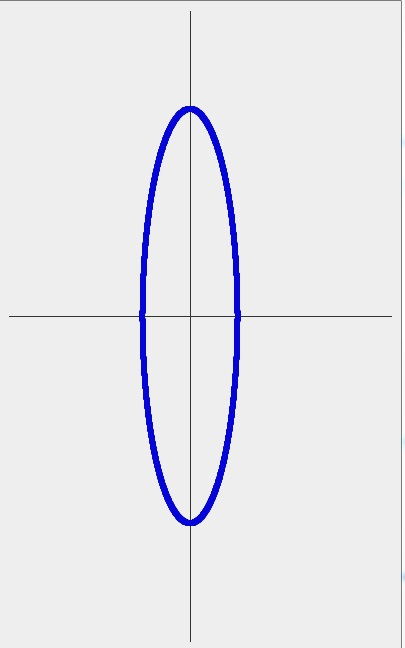
\includegraphics[width=0.3\textwidth]{side_regular_orbit_1.jpg}
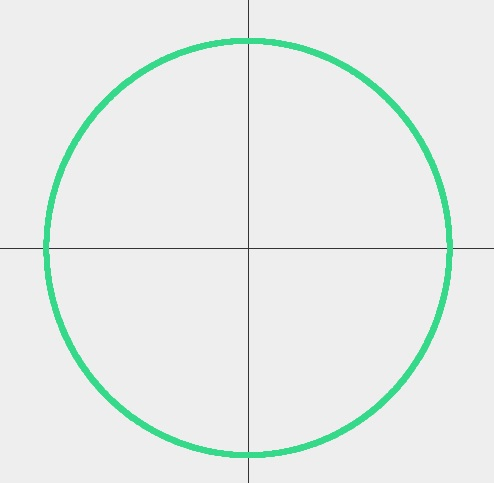
\includegraphics[width=0.3\textwidth]{side_regular_orbit_2.jpg}
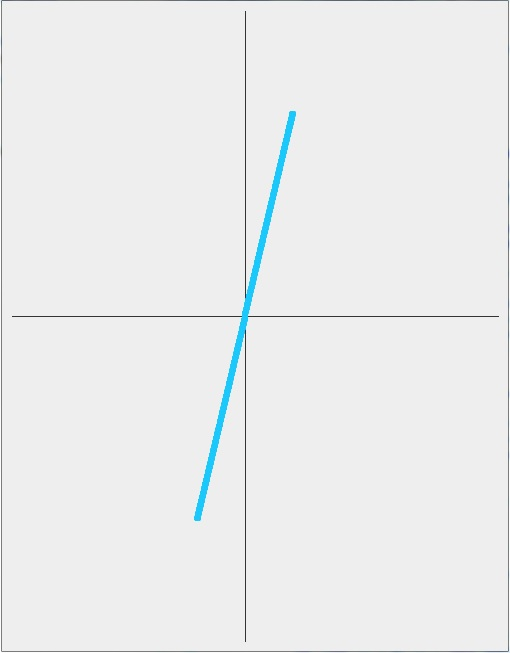
\includegraphics[width=0.3\textwidth]{top_regular_orbit.jpg}\\
Figure 1: Side and top views of paths traced by an unexploded satellite in orbit.

\end{center}
\end{figure}

\subsection{Orbital Fragmentation}

At the beginning of our trials with SORES, we simulated a satellite of mass $m_{sat}$ fragmenting into $n$ evenly sized fragments in an explosion event where $J$ kilojoules of energy are released. With the assumption that the satellite generates evenly-sized pieces of debris, the mass of each piece of debris, $m_{i}$, is given as
\begin{align}
m_{i} = m_{s} / n.
\end{align}
The kinetic energy of each fragment is therefore given as
\begin{align}
\mathit{\mathit{KE}}_{i} = \frac{1}{2}m_{i}\bar{v_{i}}^2
\end{align}
where $\bar{v_{i}}$ is the magnitude of velocity that is applied to each fragment. We assume that all the energy generated in the fragmentation event is released as kinetic energy, so
\begin{align}
J = \sum_{i = 0}^{n} \mathit{\mathit{KE}}_{i} = n \frac{1}{2} m_{i}\bar{v_{i}}^2.
\end{align}
Solving for $\bar{v_{i}}$ yields
\begin{align}
\bar{v_{i}} = \sqrt{2 J / m_{i}}.
\end{align}
The position of debris generated in a fragmentation event are initially set to the position of the satellite when the event occurred. The velocity vector of the debris fragments is set equal to the velocity vector of the satellite when the explosion takes place. The magnitude $\bar{v_{i}}$ is added to each piece of debris in a random direction. Thus, with $\vec{u_{i}}$ as a unit vector with random orientation, the velocity vector of the $i$th debris fragment, $\vec{v_i}$ is given as
\begin{align}
\vec{v_{i}} = \vec{v_{s}} + \bar{v_{i}} \vec{u_i}.
\end{align}

Figure 2 visualizes the orbit of debris generated from a single fragmentation event. As can be seen in the figure, the debris generated in a fragmentation event are left in similar, but not identical, orbits.
\begin{figure}
\begin{center}
\label{fig:sat_orbit_explosion}
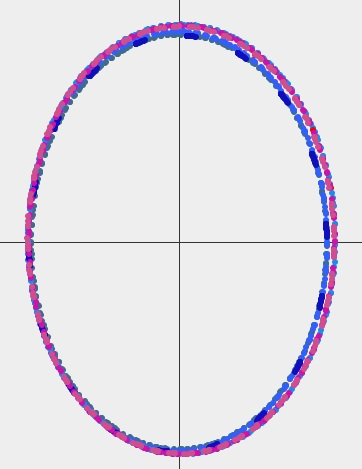
\includegraphics[width=0.4\textwidth]{depth.jpg}
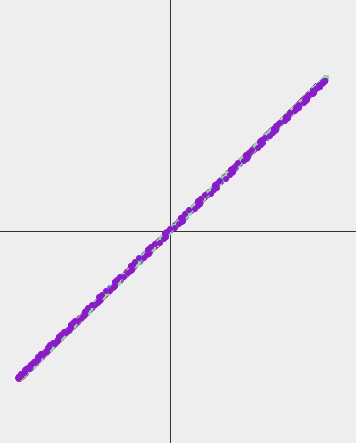
\includegraphics[width=0.4\textwidth]{top.jpg}\\
Figure 2: Side and top views of paths traced by orbital debris after a 2 kJ fragmentation event. (The plane of orbit appears skewed because is not being viewed straight-on). Debris can be observed occupying distinct orbits. 
\end{center}
\end{figure}

\subsection{SORES Mission}

After a fragmentation event, we allowed the debris fragments to circulate for $t_{w}$ before the introduction of SORES. At $t_{i} + t_{w}$, SORES was introduced into the orbit that the now-fragmented satellite originally inhabited before the explosion event, traveling in the opposite direction. The simulation continued for 100 days after the introduction of SORES. If, as checked at every time-step, orbital debris came within a distance of $r_{\mathit{eff}}$ of SORES, they were recorded as de-orbited and removed from the simulation. 

\subsection{Assessment of Conservation of Energy} \label{subsec:cons_energy}

The accuracy of any numerical analysis employing Euler's method depends on the number of iterations used, $N$. The model does not allow for energy transfer from debris once they are generated in a fragmentation event. Thus, tracking the total energy of fragments over the course of the simulation, to see whether energy is conserved, can provide a good assessment of the accuracy of the numerical simulation with $N$ iterations. Energy associated with an orbiting fragment $i$, $E_{i}$ is in the form of kinetic energy, $\mathit{KE}_{i}$, and gravitational potential energy, $\mathit{PE}_{i}$. The total energy can be given as 
\begin{align}
E_{i} 
&= \mathit{KE}_{i} + \mathit{PE}_{i} \\
&= \frac{1}{2} m_{i} \bar{v_{i}}^2 - \frac{G M_{E} m_{i}}{r}
\end{align}
where $m_{i}$ is the mass of the $i$th debris fragment.

First, we recorded the beginning and ending total energy for fifty fragments generated under standard conditions that were simulated with $N = 1\times10^{8}$ and $\ t = 7$. (These are the standard simulation conditions for the SORES delay period). The total energy of the fragments was observed to fluctuate, on average, 2.0 \% (with a standard deviation of 1.7 \%). In a second experiment, we recorded beginning versus ending kinetic energy for fifty fragments generated under standard conditions that were simulated with $N = 1\times10^{10}$ and $\Delta t = 100$ days. In this instance, the potential energy of the fragments changed by an average of 11.9 \% (with a standard deviation of 2.7 \%).\footnote{These are the standard simulation conditions for the SORES mission period.} These results suggest a mediocre, but acceptable, level of accuracy in our simulation. A sensitivity analysis of our model to the number of iterations used is provided in Section \ref{sec:sensitivity_analysis}. Our calculations were performed using Java with double floating point accuracy.

\section{Sensitivity Analysis} \label{sec:sensitivity_analysis}
We analyzed the sensitivity of our model to several variables including the number of debris fragments generated and the energy of the satellite explosion. We found significant, but not extreme, sensitivity of the model to these parameters. In particular, the results our model appears sensitive to the number of successive approximations that were used during the SORES mission, with the performance of SORES changing significantly in lower iteration trials. 
\subsection{Amount of Debris}
We found that, with SORES success defined as the percent of debris neutralized, our model was only slightly sensitive to the number of debris generated in a satellite fragmentation event, $n$. Performance of around 25 \% debris removal was observed for fragmentation events that generated 10, 25, and 50 fragments. Performance of around 40 \% debris removal was observed for 75 fragments. These results can be found in Figure 3. 
\begin{figure}
\begin{center}
\label{fig:debrisfragmentssensitivity}
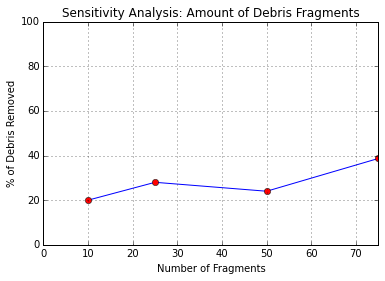
\includegraphics[width=0.7\textwidth]{fragments.png}\\
Figure 3: Results of sensitivity analysis of the performance of SORES predicted by our model to the number of debris generated in the orbital fragmentation event.
\end{center}
\end{figure}

\subsection{Explosion Energy}
In our model, the energy released during the satellite fragmentation event, $J$, affected the performance of SORES. SORES performed better cleaning up after medium-energy satellite fragmentation events, removing upwards of 35 \% of debris for 4 kJ events. For high-energy events (approximately 16 kJ), SORES performed somewhat worse, removing just over 20 \% of debris. In low-energy events, SORES fared the worst. Figure 4 presents these results. 
\begin{figure}
\begin{center}
\label{fig:explosionenergysensitivity}
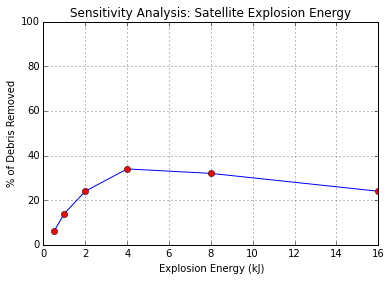
\includegraphics[width=0.7\textwidth]{energy.png}\\
Figure 4: Results of sensitivity analysis of the performance of SORES predicted by our model to the energy released in the orbital fragmentation event.
\end{center}
\end{figure}

\subsection{Iterations of Numerical Approximation}
%\end{figure}
Finally, we performed a sensitivity analysis of our model to the number of iterations of numerical approximation that were performed during the SORES mission period. As discussed in Subsection \ref{subsec:cons_energy}, the accuracy of a model employing Euler's method increases as the number of numerical approximations increases. To test the sensitivity of our results to this parameter, we ran SORES missions under standard conditions with $0.1 \times 10^{10}$, $0.5 \times 10^{10}$, and $1 \times 10^{10}$ numerical approximations between the launch of SORES and the completion of the mission. The outcomes of these trials are shown in Figure 5. We found that lowering the number of numerical approximations performed below the number used in our standard experimental setup did noticeably affect the performance of SORES predicted by our model. However, as discussed in Section 9  we are reasonably confident in the soundness of our model under the standard experimental conditions. Running tests with larger numbers of successive approximations could provide better evidence of the adequacy of the number of approximations that were used in standard conditions throughout this study, but was not feasible in the short time window the report was prepared in.
\begin{figure}
\begin{center}
\label{fig:iterationsensitivity}
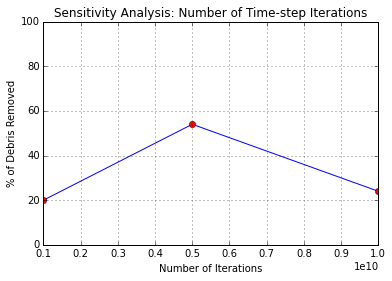
\includegraphics[width=0.7\textwidth]{iterations.png}\\
Figure 5: Results of sensitivity analysis of the performance of SORES predicted by our model to the number of iterations of each time-step.
\end{center}
\end{figure}


\section{Results} \label{sec:results}

Our primary result is the large effect that the delay in the launch of SORES has on its debris-clearing effectiveness. We found that, if launched just one day after the fragmentation event took place, under standard conditions, SORES removed upwards of 95 \% of debris if it reached orbit one day after the fragmentation event took place. With a three day delay, SORES removed slightly more than 50 \% of debris and, with a seven day delay, SORES removed approximately 25 \% of debris from orbit. At longer launch delays--20 days and 30 days--SORES de-orbited no debris. These results are presented in Figure 6. 
    
\begin{figure}
\begin{center}
\label{fig:resultsvslaunchdelay}
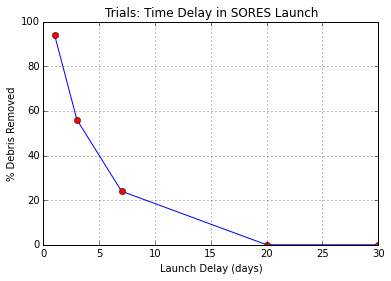
\includegraphics[width=0.7\textwidth]{delay.png}\\
Figure 6: The performance of SORES, as measured by percent debris de-orbited, tabulated over several fragmentation-to-launch delays.
\end{center}
\end{figure}
    
It is likely that with strategic orbit choice based on updated telemetry data on debris, the effectiveness of a SORES launch at longer delay could be somewhat increased. In our simulation, SORES was simply launched into the orbit of the satellite that fragmented; perhaps a smaller cluster of debris in a nearby orbit could be targeted by SORES. However, even with these adjustments, the performance of SORES is likely to be highly dependent on how soon after the fragmentation event the SORES neutralization mission begins due to the dispersal of fragment orbits over time.
    
We found that an effective radius of around 1 km is necessary for any de-orbiting of debris. Our results showed, as would be expected, that a larger radius of effect led to more debris de-orbited. Below a 1 km effective radius, no debris removal was observed. Figure 7 shows the relationship between SORES effective radius and debris de-orbited suggested by our model. It should be noted, however, that if a craft could be launched soon after a fragmentation event, our findings in Figure 6 suggest that it could have a large effect even with a smaller effective radius.
\begin{figure}
\begin{center}
\label{fig:resultsvseffectiveradius}
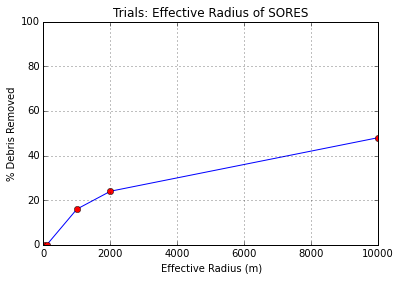
\includegraphics[width=0.7\textwidth]{radius.png}\\
Figure 7: The relationship of SORES effective radius and its success at de-orbiting space debris.
\end{center}
\end{figure}

We found that our the  model was somewhat sensitive to the altitude at which the fragmentation event took place. The results of this analysis are shown in Figure 8. Our model predicted better performance for SORES missions to neutralize fragmentation events that take place in very low-altitude orbit. Altitude changes between mid LEO and MEO (900 to 3000 km) had a small and inconsistent effect on the performance of SORES.
    
\begin{figure}
\begin{center}
\label{fig:altitudesensitivity}
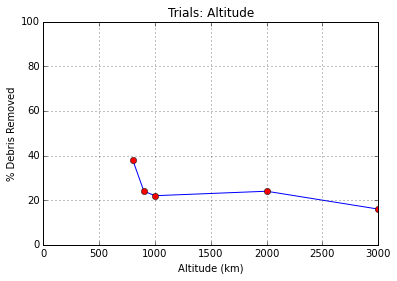
\includegraphics[width=0.7\textwidth]{altitude.png}\\
Figure 8: SORES performance tabulated over a orbital altitudes ranging from LEO to mid MEO.
\end{center}
\end{figure}
    
Although our model predicts the best SORES performance for medium intensity fragmentation events, it is likely that in actuality this is presumably because the debris cluster is not spread out enough to have a significant likelihood of interacting with SORES. In this case SORES could likely be navigated to hit the debris cluster. However, SORES is likely to perform poorly in high-energy fragmentation events such as collisions because the wide dispersal of debris cannot be overcome by better targeting.

However, our simulations do not indicate large risk of debris impact with SORES. Missions with 1 day and 1 week SORES launch delays, simulated three times each, found no instances of SORES encountering space junk at a distance of less than 10 m. However, as discussed in Subsection \ref{subsec:risk_assessment}, this result in a small number of simulations does not provide adequate evidence of the safety of a SORES mission (in particular, with SORES traveling in the opposite direction of debris that it is neutralizing there is a potential for head-on collision).

\section{Model Assessment} \label{sec:model_assessment}
\subsection{Strengths}
    \begin{itemize}
        \item The model simulates orbital mechanics to an adequate accuracy, as assessed by visual analysis of orbit path and mathematical evaluation of conservation of energy in the model.
        \item The model provides a simple, but reasonable, simulation of satellite fragmentation in three dimensions over a short time period.
        \item The model successfully assesses the number of debris de-orbited by a SORES satellite, with this success count responding to changes in parameters (such as SORES effective radius and delay before SORES launch) as would be expected.
    \end{itemize}
\subsection{Weaknesses}
    \begin{itemize}
        \item The model is computationally intensive, with computational costs scaling linearly both with number of fragments and mission duration. These costs make long-term simulation of large numbers of debris infeasible.
        \item The model neglects drag effects, the non-uniformity of Earth's gravitational field, and the gravitational interference of other celestial bodies. These effects are negligible for simulations of short time-periods, but their absence may affect longer term simulations.
        \item Most experimental results were derived from a single trial, which casts some uncertainty on their reproducibility.
    \end{itemize}
\subsection{Improvements}
    \begin{itemize}
        \item Parallel computing techniques should be employed to reduce the computational costs of simulating our model.
        \item Experimental results should be derived from a battery of independent simulation trials.
        \item The model should be extended to extended to specifically consider orbital collision events, in addition to orbital explosion events.
        \item The satellite fragmentation and orbital mechanics models should be compared to empirical data and be further developed and refined.
    \end{itemize}
\section{Discussion} \label{sec:discussion}
\subsection{Risk Assessment} \label{subsec:risk_assessment}
NASA quantifies risk to a mission as the probability of a collision multiplied by the consequence \cite{risk}. For a critical debris removal mission there are three pieces to the overall risk, following from NASA's quantization model.
\subsubsection{Baseline Risk}
The baseline risk of a satellite. They are typically insured (see cost analysis section below) and that coverage currently includes damage due to debris and loss of control due to other circumstances. However, as the frequency of minor to catastrophic damage caused by debris rapidly increases, the insurance companies will eventually drop their coverage. This in turn will significantly reduce the incentive for private companies to invest in removal strategies as there will be heavy additional costs and associated risks.
\subsubsection{Debris Risk}
The increased risk of damage by debris. The probability of an impact at 800-900 km altitude in the LEO with debris larger than 1 cm is \(0.12\) \(\%\) for a 100 day lifespan \cite{risk}. However, this value is for a maneuverable satellite in an orbit designed to avoid cataloged debris. The orbit of SORES on the other hand, is designed to hit the highest concentration of debris density. This significantly increases the risk of a collision if we remove our original assumption that SORES performs perfectly in the removal of debris. Modeling this possibility with an effective radius of 1 m with otherwise standard conditions and 5 repetitions resulted in no collisions with debris.\footnote{For accurate modelling of this effect, more repetitions of the simulation are needed.} There is also the risk that SORES encounters an object that is too big for it do deal with, causing potentially fatal damage. However, this is dependent on the individual removal techniques and is beyond the scope of this model. We can say that like a typical satellite, SORES is designed to withstand impact from debris. This makes the debris associated risks substantially less probable than launch or mechanical failure.
\subsubsection{Legal Risk}
Finally there is a legal risk. Permission from the owner of the debris fragment being removed from space must be given. The possibility of debris reaching the surface must be considered as it could cause damage or injury, as most debris removal techniques do not control the re-entry of the debris.

\subsection{Cost Analysis}
\subsubsection{Cost Assumptions}
\begin{itemize}
\item	We use the straight line depreciation method to analyze the value of a satellite.
\item	We do not time value the money; we neglect the possible lost investment.
\item   Insurance on the satellites only covers damage caused by space debris.
\item	We neglect the cost of launching the satellites.
\item	There are approximately 277 debris fragments in each two-dimensional orbit at 900 km altitude.\footnote{From the density of debris at that altitude\cite{fragments} stated in the Background section and the circumference of the Earth, \[\sqrt[3]{4.55 \times 10^{-8}}(2\pi r_E)=163 \text{ fragments per orbit.}\] Then using NASA's publication on the history of satellite fragmentation \cite{fragments}, the number of fragments per documented collision in the LEO, we calculated the mean to be 114 per collision. Thus \(163+114=277\) debris fragments.}
\item   The individual risk potential for each debris fragment is not considered; each fragment is treated as the same amount of risk to a satellite.
\end{itemize}
\subsubsection{Variables and Parameters}
\begin{itemize}
    \item \(c_t\): the total cost of a 20 year mission; \(\$200\) million.
    \item \(c_I\): the amount covered by the insurance company; \(\$129\) million.
    \item \(p_c\): the probability of a collision between a satellite and a debris fragment in 1 year; 0.006.
    \item \(s\): the number of satellites in LEO; 1000 satellites.
    \item \(n_L\): the amount of debris larger than 1 cm in LEO; 377,600 objects.
\end{itemize}

\subsubsection{Total Costs}
In itself the cost of a launch is about \(\$50-\$100\) million for a mid-sized satellite. Then everything else costs up to \(\$290\) million with a development and production time of 1-4 years \cite{cost}. The estimate can be further broken down into the phases of the mission to get a better picture of when money is spent. There are four phases:
\begin{enumerate}
    \item Technology and concept development
    \item Research, development, test and evaluation
    \item Production
    \item Operations.
\end{enumerate}

It is important to note that most methods of cost estimation do not take into account the development of technology. Parametric estimation is one method that is frequently used, which utilizes the cost estimating relationship that relies on past projects for data \cite{cost}. When estimating cost inflation must be taken into account. It is also important to separate the fixed and recurring costs in an estimate.

%We assume that the private company owning the debris removing satellite will operate in a cost effective manner. The facility cost could be mitigated by using contractors for the launch site construction, as well as foregoing the use of a communications tower for satellite communication. The insurance company might possibly be convinced to pay for the cleanup of the testing and production of the satellite in exchange for covering the lost investment if the satellite was destroyed in orbit. Another option is to share the launch with a second company to help off-set the costs.

\subsubsection{Bounties}
Insurance companies cover satellites for an average of \(\$129\) million for catastrophic failure events, including damage from debris \cite{cost}. Therefore, they are directly affected by the increasing amount of debris. Following the assumptions above, the total cost to the insurance company due to debris is 
\[c_I \cdot p_c \cdot s = \$774\text{ million}.\]
Then, the "bounty" on a single piece of debris in the LEO is
\[\frac{\$774\text{ million}}{n_L}=\$2050.\]
Assume the cost of a mid-sized debris removal satellite with a functional lifespan of 20 years, including relaunches, is \(\$200\) million. Using straight line depreciation to break even on debts and investments, the company would need to make about \(\$10\) million per year from that satellite. Therefore they would need to collect the bounties on 
\[\frac{\$10\text{ million}}{\$2050}=4880\text{ debris fragments}\]
to break even. So the company would need to remove a minimum of 4880 pieces of debris per year to stay out of debt, assuming the space cleanup mission were their only source of income.

The number of debris that would need to be captured over the lifetime of the SORES mission is much greater than the amount of debris generated by a single collision, which is only 114 fragments. \cite{excel} Thus, such a mission would not currently be viable.

A SORES mission may become viable a few years down the road. Advances in the private rocketry industry promise to drastically reduce the cost of launch. Additionally, increasing density of objects in low earth orbit (both junk and functional satellites) might raise the risk of knock-on fragment generation and the number of preexisting debris that are encountered to the point where the benefits of a SORES cleanup operation, perhaps with the support of government grant money, might outstrip the costs. 

\subsection{Mechanisms of SORES}
From the model, SORES needs approximately a 1 km radius of effect. As discussed in the Introduction, there are multiple proposed mechanism designs that are in various stages of development and testing. If they are able to generate the required effective radius, then their design fits all the requirements for a SORES satellite and are thus a viable solution to the orbital debris problem. The possibilities to capture the debris are
\begin{itemize}
    \item GRASP: a mid-sized satellite with a cage-like arm \cite{tether},
    \item NanoSail-d: a micro-satellite that deploys a sail \cite{sail},
    \item A mid-sized satellite that deploys nets \cite{net}.
\end{itemize}
The calculated effective radius could alternately be an  active guidance system on the satellite or come from a ranged effect from puffs of gas or lasers.

\section{Recommendations} \label{sec:recommendations}
\begin{itemize}
    \item SORES needs to be maneuverable and/or structurally robust to impact with debris, in order to minimize risk and consequence of potential collisions with space debris. A more comprehensive risk assessment must be undertaken before proceeding with a SORES mission, and a SORES probe should be designed with this risk in mind.
    \item Our models predict that SORES type missions are more successful at remedying low-altitude fragmentation events. Coupled with the fact that the greatest concentration of satellites is in LEO, which would be threatened by low-altitude debris, a SORES mission is more likely to pencil out for a low-altitude fragmentation event.
    \item To maximize the effectiveness of a SORES mission, minimizing the time that passes between a fragmentation event and launch is key. A SORES mission will be most effective if it is kept on standby until such an event occurs. If the fragmentation to launch time frame could be reduced to less than a week, a SORES approach could potentially be very effective. 
    \item The effectiveness of a SORES mission also depends on the effective radius of debris capture of the probe. This radius should be, at a minimum, around 1km. Such a radius of effect could potentially be implemented through a solar sail-type debris net coupled with an active guidance system or by a ranged effect such as gas puffs or lasers.
    \item Our cost assessments suggest that a SORES-type intervention is not currently economically feasible. However, if the space debris situation deteriorates significantly, this type of intervention may become palatable.
\end{itemize}

\section{References}


\begingroup
\renewcommand{\section}[2]{}%
\begin{thebibliography}{50}

\bibitem{1995 IA} 
United States. Office of Science and Technology Policy. Transportation Research and Development. \textit{Interagency Report on Orbital Debris 1995}. NASA Orbital Debris Program Office. Web. 29 Jan. 2016.
\bibitem{ESA} 
"Space Debris." \textit{European Space Agency}. 19 Apr. 2013. Web. 31 Jan. 2016.
\bibitem{ODPO}
\textit{"NASA Orbital Debris Program Office."} NASA Orbital Debris Program Office. Web. 29 Jan. 2016.
\bibitem{solar cycle}
Hathaway, Dr. David. "Solar Cycle Prediction." \textit{Solar Physics}. Marshall Space Flight Center and NASA, 12 Jan. 2016. Web. 29 Jan. 2016.
\bibitem{UN}
United Nations. \textit{Technical Report on Space Debris}. NASA Orbital Debris Program Office, 1999. Web. 29 Jan. 2016.
\bibitem{excel}
\textit{UCS Satellite Database 9-1-15.} Union of Concerned Scientists, 1 Sept. 2015. Excel.
\bibitem{punch}
Redd, Nola Taylor. "Space Junk: Tracking \& Removing Orbital Debris." \textit{Space.com}. 8 Mar. 2013. Web. 31 Jan. 2016.
\bibitem{model}
Bordovitsyna, T. V., and A. G. Aleksandrova. "Numerical Modeling of the Formation, Orbital Evolution, and Distribution of Fragments of Space Debris in Near-Earth Space." \textit{Solar System Research} 44.3 (2010): 238-51. Web. 30 Jan. 2016.
\bibitem{boom}
Pardini, C., L. Anselmo, A. Rossi, A. Cordelli, P. Farinella. \textit{The 1997.0 CNUCE Orbital Debris Reference Model.} 8th AAS/AIAA Space Flight Mechanics Meeting, 1997. Web. 29 Jan. 2016. 
\bibitem{fragments}
United States. NASA. Orbital Debris Program. \textit{History of On-Orbit Satellite Fragmentations}. NASA Orbital Debris Program Office, June 2008. Web. 29 Jan. 2016.
\bibitem{cost}
Miller, David W., John Keesee, and Cyrus Jilla. \textit{Space Systems Cost Modeling.} Massachusetts Institute of Technology, Sept. 2003. PPT.
\bibitem{risk}
Bensoussan, Denis. \textit{Satellite Vulnerability to Space Debris Risk.} Dubai: World Space Risk Forum, 2012. PPT.
\bibitem{cost}
Vidyakin, Ivan. "How Much Would It Cost to Build a Private Satellite Network?" - Quora. Web. 31 Jan. 2016.
\bibitem{insurance}
"Covering Satellite Risks." Satellite Insurance and Space Risks. Web. 31 Jan. 2016.
\bibitem{tether}
"Grapple, Retrieve, and Secure Payload (GRASP)." \textit{Tethers Unlimited}. Web. 30 Jan. 2016.
\bibitem{sail}
Dunbar, Brian. "NASA's Nanosail-D 'Sails' Home -- Mission Complete." \textit{Small Satellite Missions}. NASA, 29 Nov. 2011. Web. 31 Jan. 2016.
\bibitem{net}
"Want to Snag a Satellite? Try a Net." \textit{Clean Space}. European Space Agency. Web. 30 Jan. 2016.
\end{thebibliography}
\endgroup

\end{document}
